Each of the models presented indicate that the GSN framework is suitable for learning useful representations of complex sequential input data. The results are summarized below and compared to the RNN-RBM and RTRBM models discussed in Chapter 2 (Related Work).

\section{Samples from RNN-RBM on sequenced MNIST}

Compared to the samples generated by the RNN-RBM, it is clear that the GSN framework has an easier time mixing between modes of the input data. It also appears to form better reconstructions of the input data. This improvement can be attributed to a deeper representation of the input space, since the RNN-RBM only had two layers - one for the RBM and one for the RNN.

\begin{figure}[h!]
  \centering
    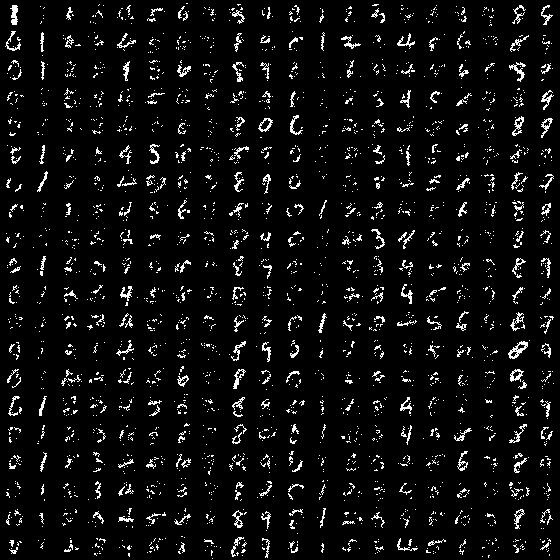
\includegraphics[width=0.8\textwidth]{rnnrbm_samples}
\caption{RNN-RBM sampling after 300 iterations.}
\end{figure}

\section{Bouncing balls videos dataset}

This dataset generates videos of 3 balls bouncing and colliding in a box as described in \cite{lewandowski12}\footnote{http://www.cs.utoronto.ca/~ilya/code/2008/RTRBM.tar}. The videos have length of 128 frames with 15x15 resolution of pixels in the range of [0, 1]. Training examples are generated artificially at runtime so each sequence seen is unique, which helps reduce overfitting.

\section{CMU motion capture dataset}

This dataset is a series of captured human joint angles, translations and rotations around the base of a spine as in \cite{sutskever08}\footnote{https://github.com/sidsig/NIPS-2014}. There are 3826 samples of 49 real-valued inputs, so input sampling was not used for the GSN and the visible layer had a linear activation.

\begin{table}[h!]
\begin{tabular*}{\textwidth}{p{4cm} r r r r}
\hlinewd{1.5pt}
  & Bouncing Balls & CMU Motion Capture \\
\hline
LSTM & training... & training...\\
RTRBM & 2.11 & 20.1\\
RNN-RBM & 0.96 & 16.2\\
Untied GSN & training... & training...\\
TGSN & training... & training...\\
RNN-GSN & training... & training...\\
SEN & training... & training...\\
\hlinewd{1.5pt}
\end{tabular*}
\caption{Mean squared prediction error on bouncing balls videos and motion capture data. RTRBM and RNN-RBM numbers from [10]}
\end{table}


